% ------------------------------------------------------------
\section{Calendar Week}
% ------------------------------------------------------------
% --------------------------------------------------- Slide --
\subsection{CW 40}
% ------------------------------------------------------------
\begin{frame}
  \frametitle{Review CW 40}
	\begin{itemize}
		\item Compared solution of first Finite Element simple model with analytical solution calculated "by hand". "Hand" calculation performed with math software Blockpad. Results matched for single case, providing confidence that at least simple model is working correctly. \textcolor{green}{Done}
		\item FEA Model with Titanium alloy (Ti-6Al-4V) developed for fatigue calculation for single test case. Similar to last week, but there it was used structural steel. SN curves from literature (paper from Janecek2015) used as reference. Only damage calculated for a single case at first. It correctly compared with the "hand"/analytical calculation above. \textcolor{yellow}{In-Work}
	\end{itemize}
\end{frame}

\begin{frame}
  \frametitle{Review CW 40 - Comparison "Hand" vs FEA Calculation}
	\begin{figure}
		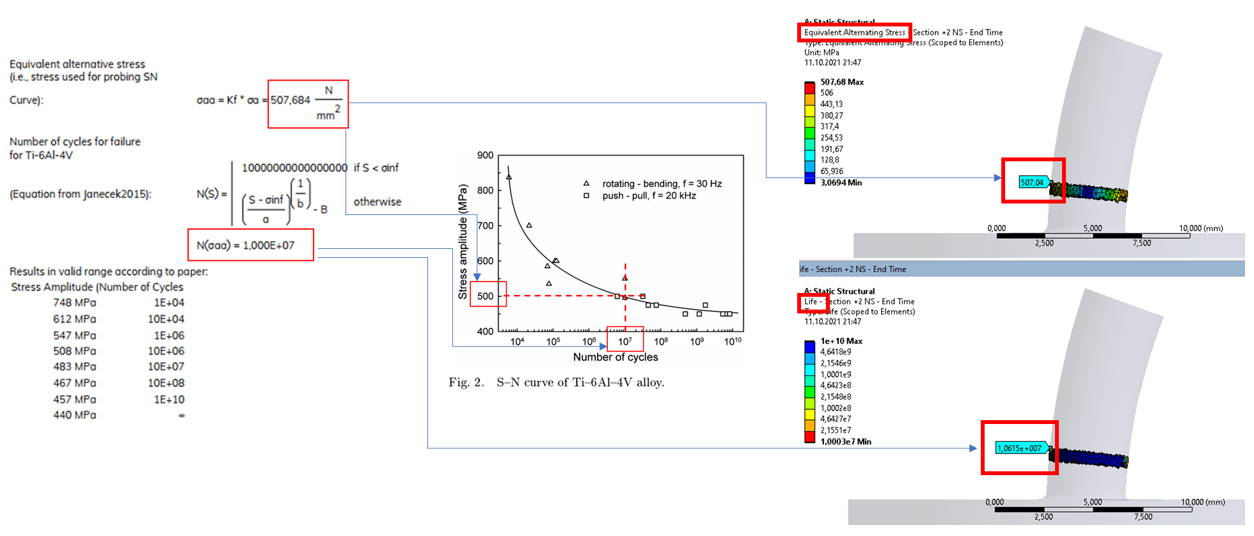
\includegraphics[width=1.0\textwidth]{pictures/CW40}
	\end{figure}
	\centering Analytical calculation (Left) vs. FEA (right).
	
	\centering In the middle, the SN curve from Janecek2015 is shown.
\end{frame}

% ------------------------------------------------------------
% --------------------------------------------------- Slide --
\subsection{CW 41}
% ------------------------------------------------------------
% ------------------------------------------------------------
\begin{frame}
  \frametitle{Outlook CW 41}
	\begin{itemize}
		\item Continue to develop fatigue calculation for test case (even simpler geometry at first), but now with different cases (i.e., increasing beam (simplified implant)) length due to peri-implantitis. 
		\item Idea is to use a similar profile of different conditions as done the previous week (see table below repeated only for reference).
	\end{itemize}
	\begin{center}
	\begin{tabular}{|c|c|c|} 
 		\hline
 		Year & Damage of bone(mm) & Number of cycles\\ 
 		0  & 0 & 1.25 million \\ 
 		5  & 1 & 1.25 million \\ 
 		10 & 2 & 1.25 million \\ 
 		15 & 3 & 1.25 million \\ 
		\hline
	\end{tabular}
	\end{center}
\end{frame}
% --------------------------------------------------- Slide --

